\section{Figure excerpts from documentation sources}
\begin{figure}[H]
    \centering
    \begin{subfigure}[b]{0.5\textwidth}
         \centering
         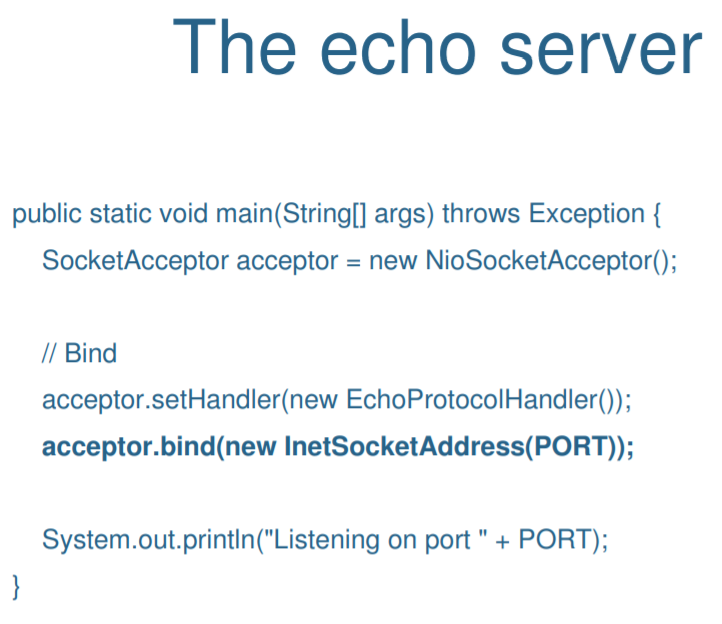
\includegraphics[width=\textwidth]{images/usability_extensibility1.png}
     \end{subfigure}
   
     \begin{subfigure}[b]{0.5\textwidth}
         \centering
         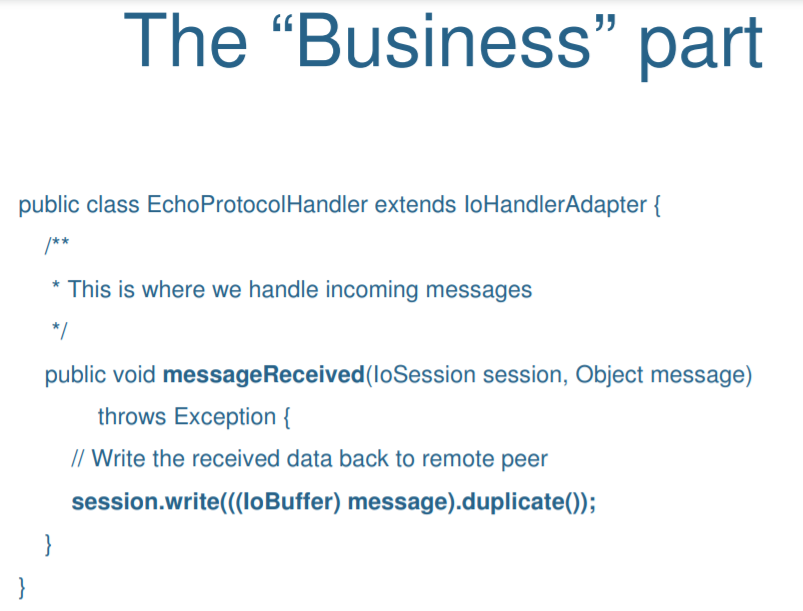
\includegraphics[width=\textwidth]{images/usability_extensibility2.png}
     \end{subfigure}
   
    \begin{subfigure}[b]{0.5\textwidth}
         \centering
         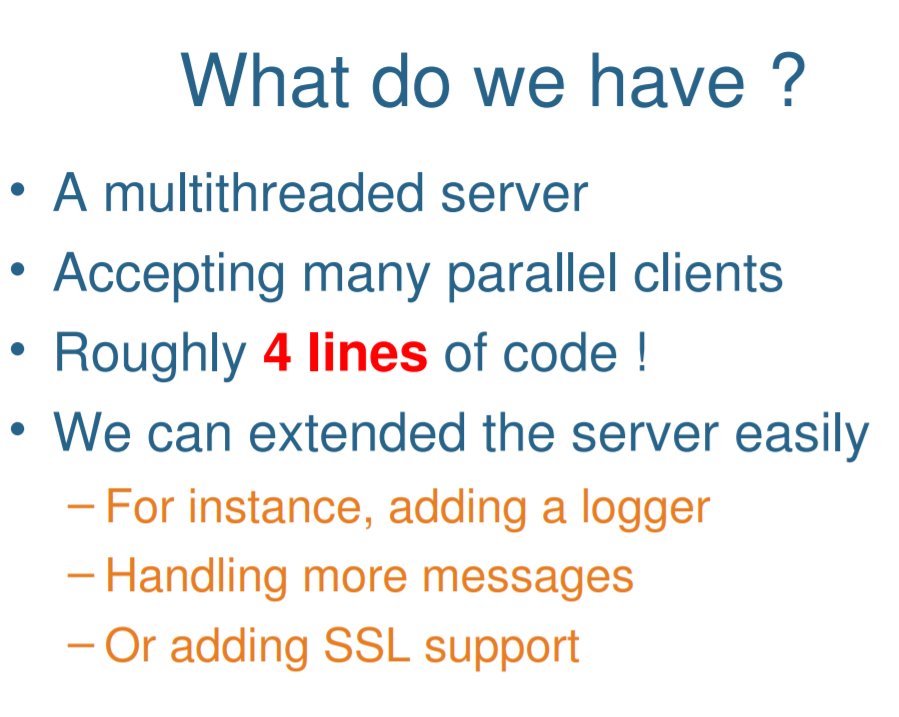
\includegraphics[width=\textwidth]{images/usability_extensibility.png}
     \end{subfigure}
    
    \caption{An exercept from \cite{mina-talk2009} that showcases the ease of use and extensibility of the MINA framework.}
    \label{fig:usability_extensibility}
\end{figure}

\begin{figure}[H]
    \centering
    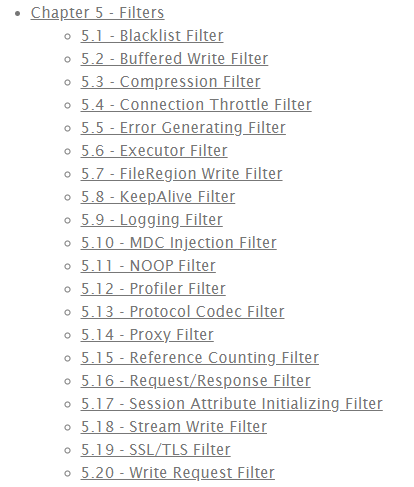
\includegraphics[width=0.6\textwidth]{images/filters.png}
    \caption{An overview of the out-of-the-box filters offered by the MINA framework; the overview has been extracted from \cite{mina-userguide}.}
    \label{fig:filters}
\end{figure}

\begin{figure}[H]
    \centering
    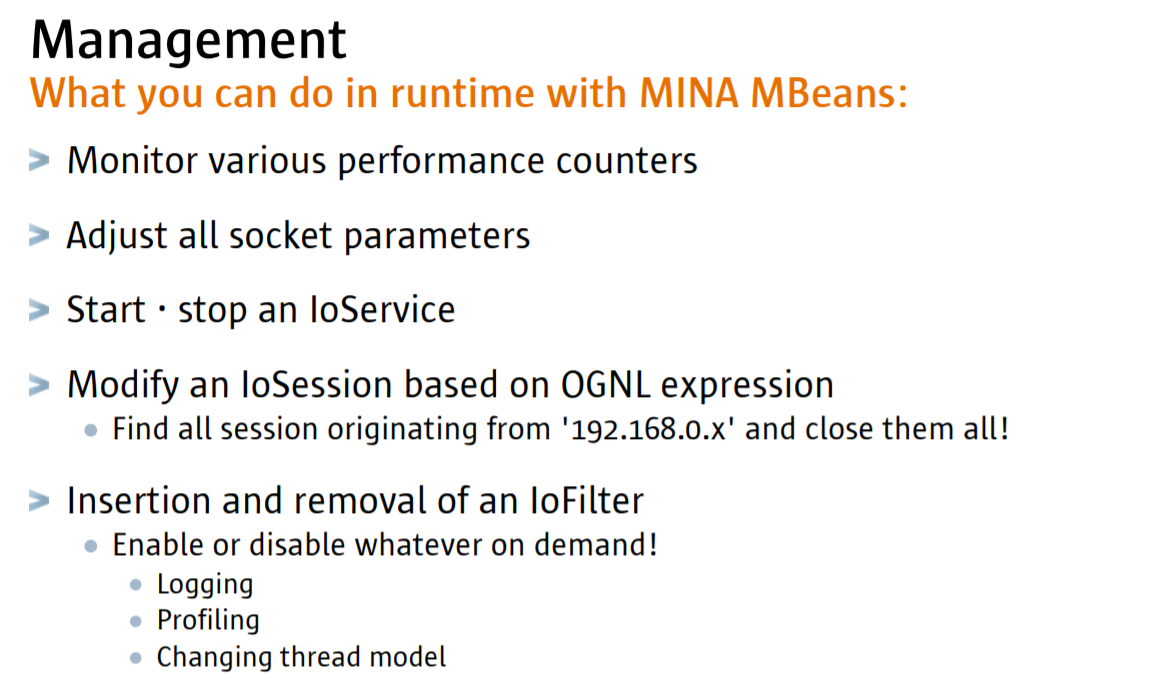
\includegraphics[width=0.7\textwidth]{images/management.png}
    \caption{Excerpt from \cite{mina-talk2008} showing the runtime management capabilities of MINA applications integrated with JMX.}
    \label{fig:manageability}
\end{figure}

\begin{figure}[H]
    \centering
    \begin{subfigure}[b]{0.7\textwidth}
         \centering
         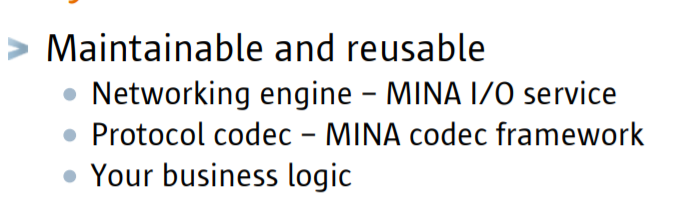
\includegraphics[width=\textwidth]{images/reusable1.png}
     \end{subfigure}

     \begin{subfigure}[b]{0.7\textwidth}
         \centering
         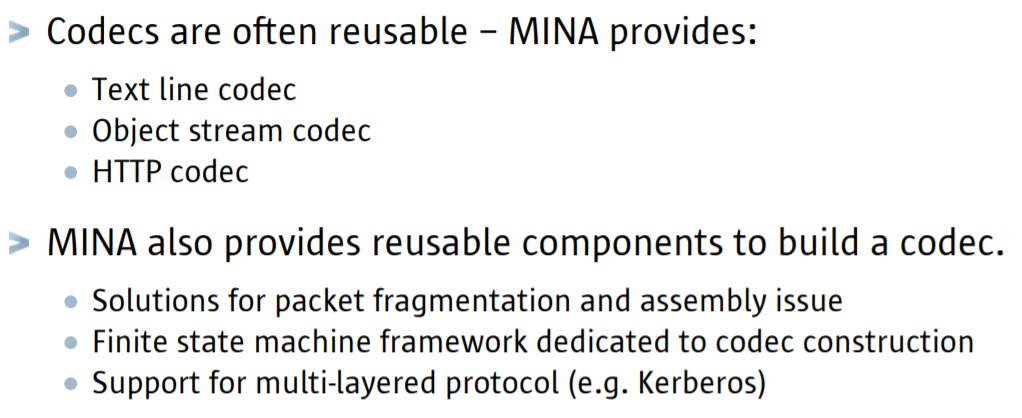
\includegraphics[width=\textwidth]{images/reusable.png}
     \end{subfigure}
     
    \begin{subfigure}[b]{0.7\textwidth}
         \centering
         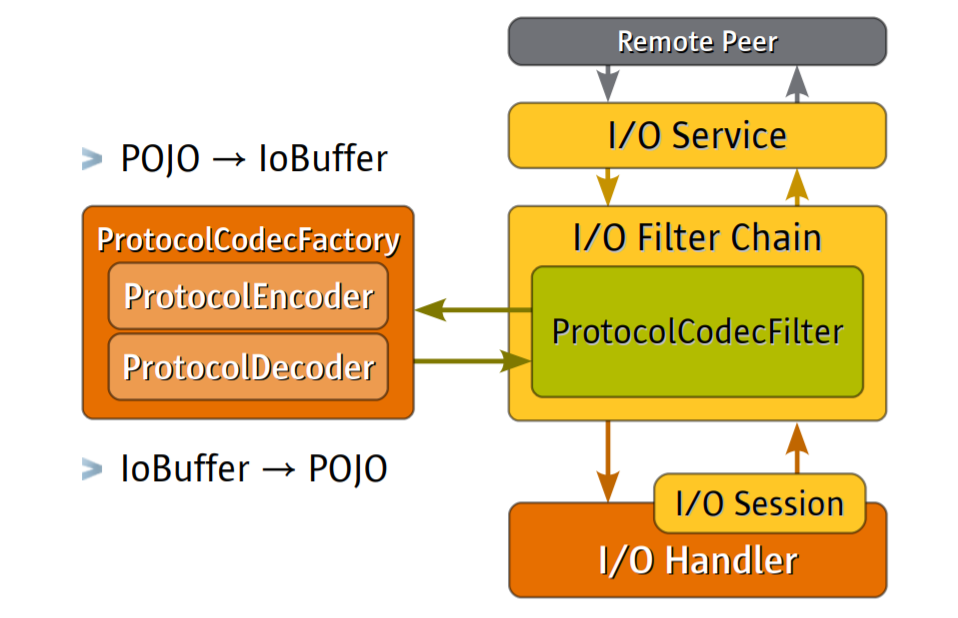
\includegraphics[width=\textwidth]{images/architecture_codec.png}
     \end{subfigure}
    
    \caption{An exercept from the presentation \cite{mina-talk2008} that showcases the high reusability  of components from the MINA framework.}
    \label{fig:reusability}
\end{figure}
\newpage
\section{Overview of the high-level architecture}

\begin{landscape}
\begin{figure}
    \centering
    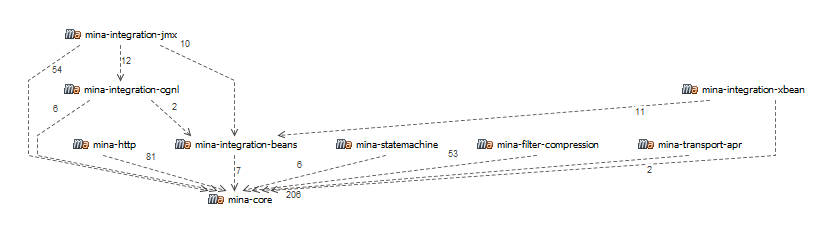
\includegraphics[scale=0.9]{images/MINA_package_dependencies.png}
    \caption{High-level overview of the MINA packages and their dependencies}
    \label{fig:overview_package_dependencies}
\end{figure}
\end{landscape}

\section{Overview of architectural components}
\subsection{MINA core}
\begin{figure}[H]
    \centering
    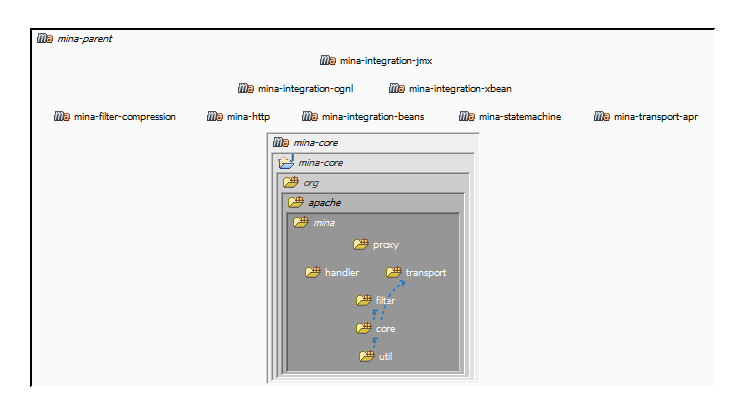
\includegraphics[width=\textwidth]{images/MINA_core_initial.png}
    \caption{Initial high-level structure of the \texttt{mina-core} module.}
    \label{fig:mina_core_initial}
\end{figure}

\begin{figure}[H]
    \centering
    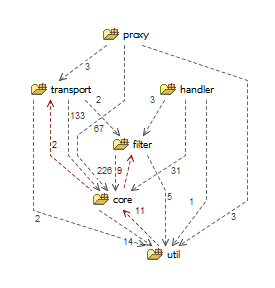
\includegraphics{images/MINA_core_initial_dependencies.png}
    \caption{Initial high-level dependency graph of the \texttt{mina-core} module}.
    \label{fig:mina_core_dependencies_initial}
\end{figure}

\begin{figure}[H]
    \centering
    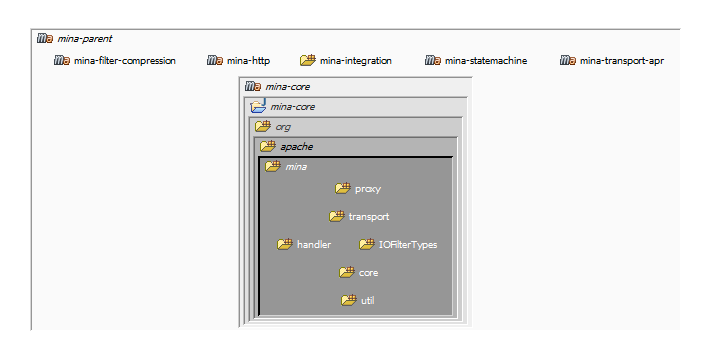
\includegraphics[width=\textwidth]{images/MINA_core_restructure.png}
    \caption{High-level structure of the \texttt{mina-core} module after restructuring.}
    \label{fig:mina_core_restructured}
\end{figure}

\begin{figure}[H]
    \centering
    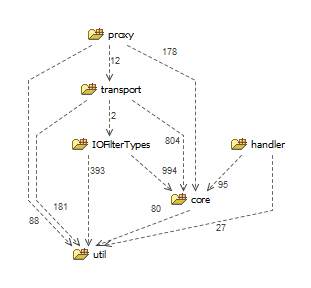
\includegraphics{images/MINA_core_dependencies_restructure.png}
    \caption{High-level dependency graph of the \texttt{mina-core} module after restructuring.}
    \label{fig:mina_core_dependencies_restructured}
\end{figure}

\begin{landscape}
\begin{figure}
    \centering
    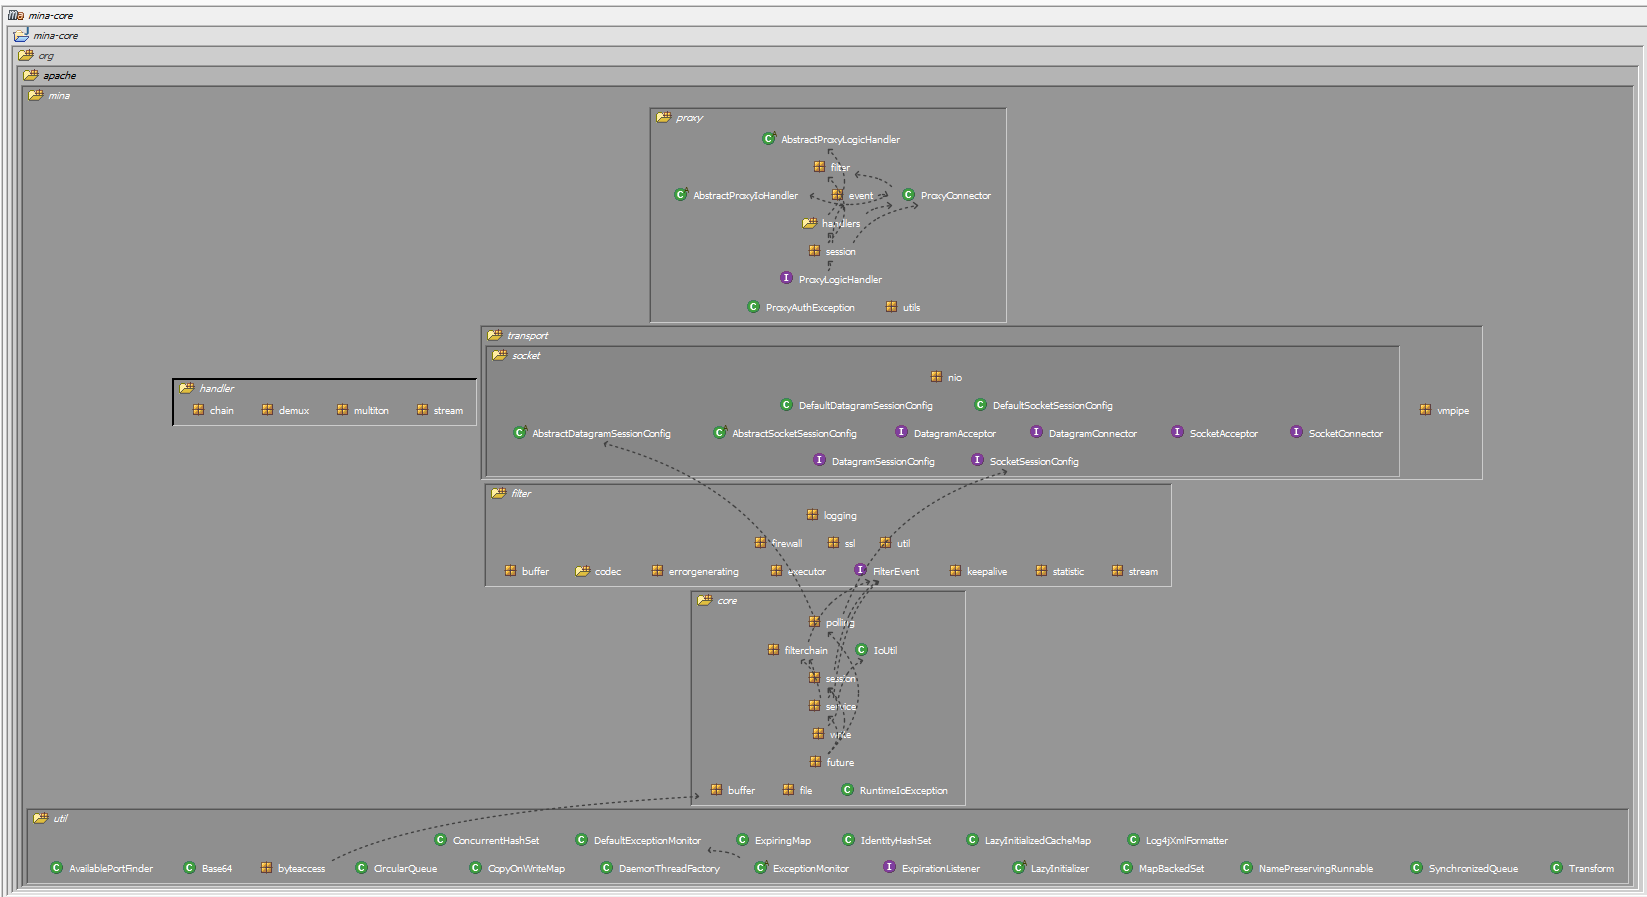
\includegraphics[width=\linewidth]{images/MINA_core_extended_initial.png}
    \caption{Detailed view of \texttt{mina-core} module.}
    \label{fig:mina_core_initial_detailed}
\end{figure}
\end{landscape}

\begin{landscape}
\begin{figure}
    \centering
    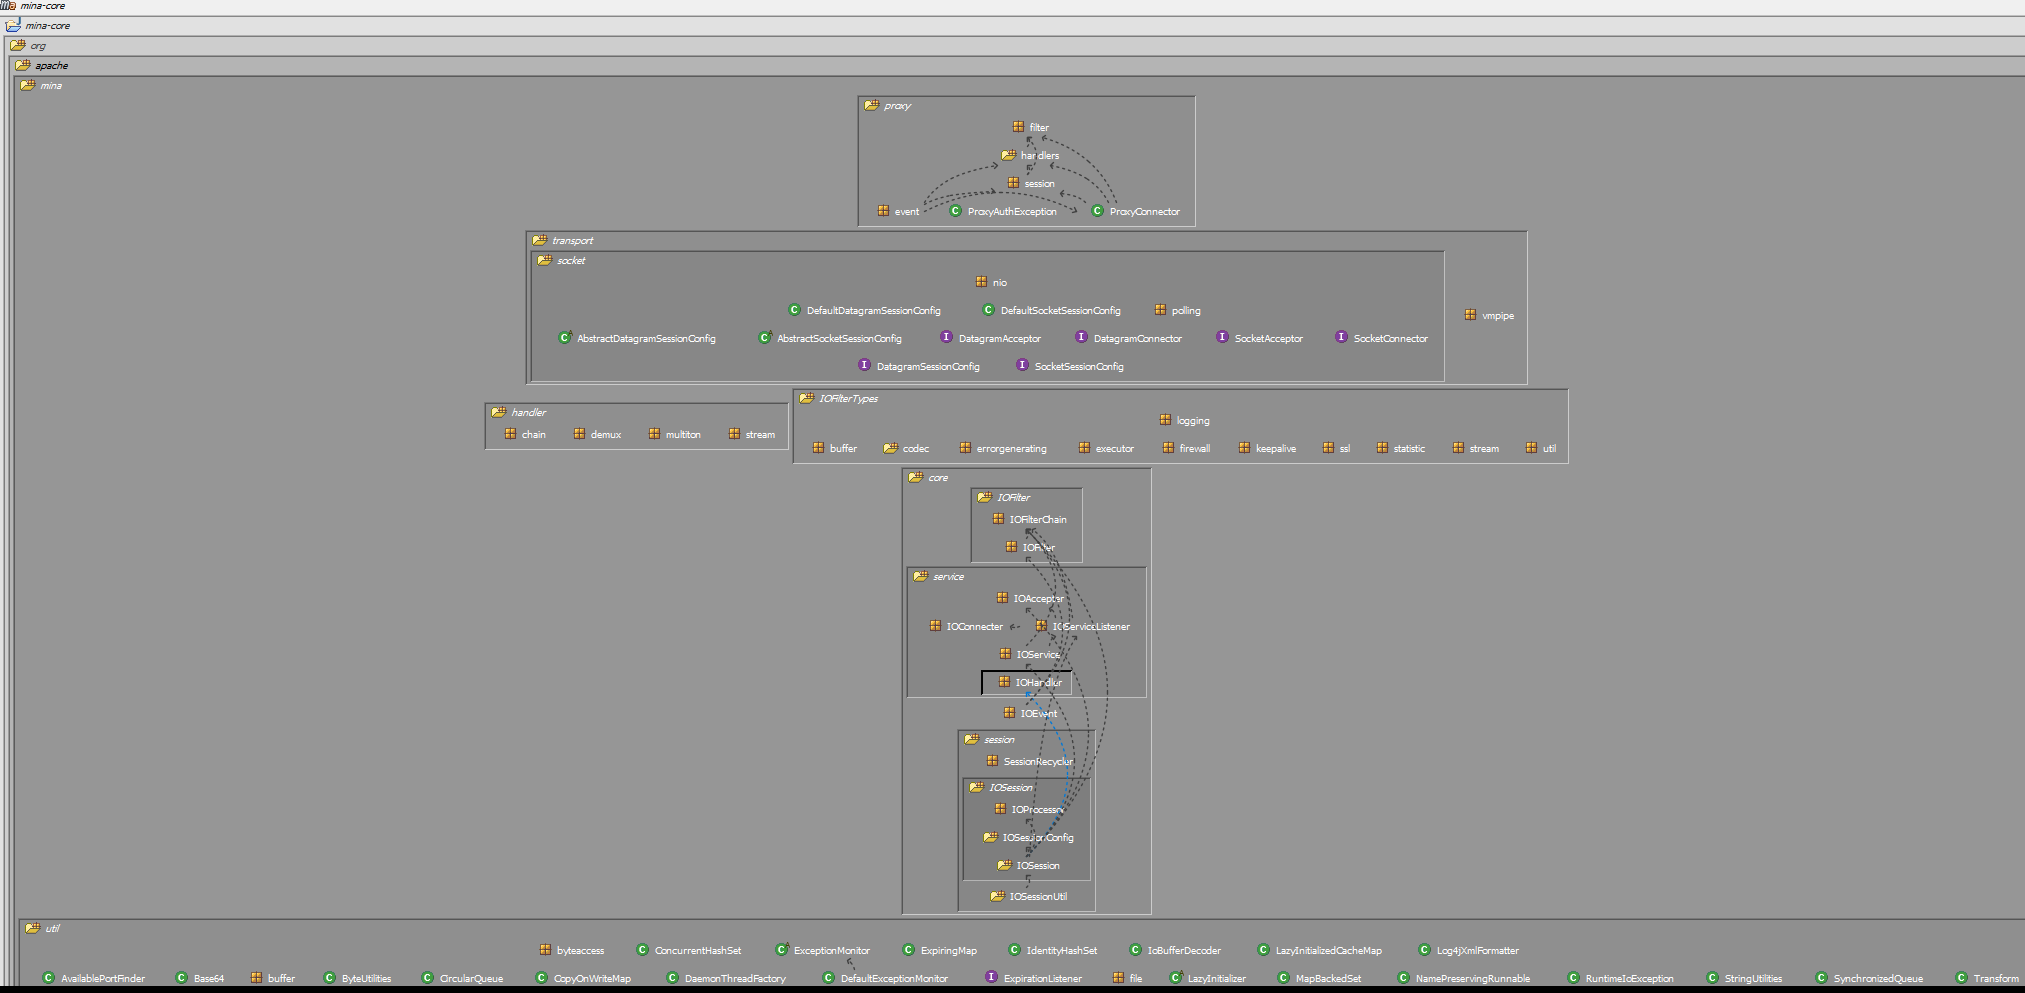
\includegraphics[scale=0.4]{images/MINA_core_extended_restructured.png}
    \caption{Detailed view of the restructured \texttt{mina-core} module.}
    %\label{fig:mina_core_initial_detailed}
\end{figure}
\end{landscape}

\subsubsection{MINA \texttt{core} component from the core module}

\begin{figure}[H]
    \centering
    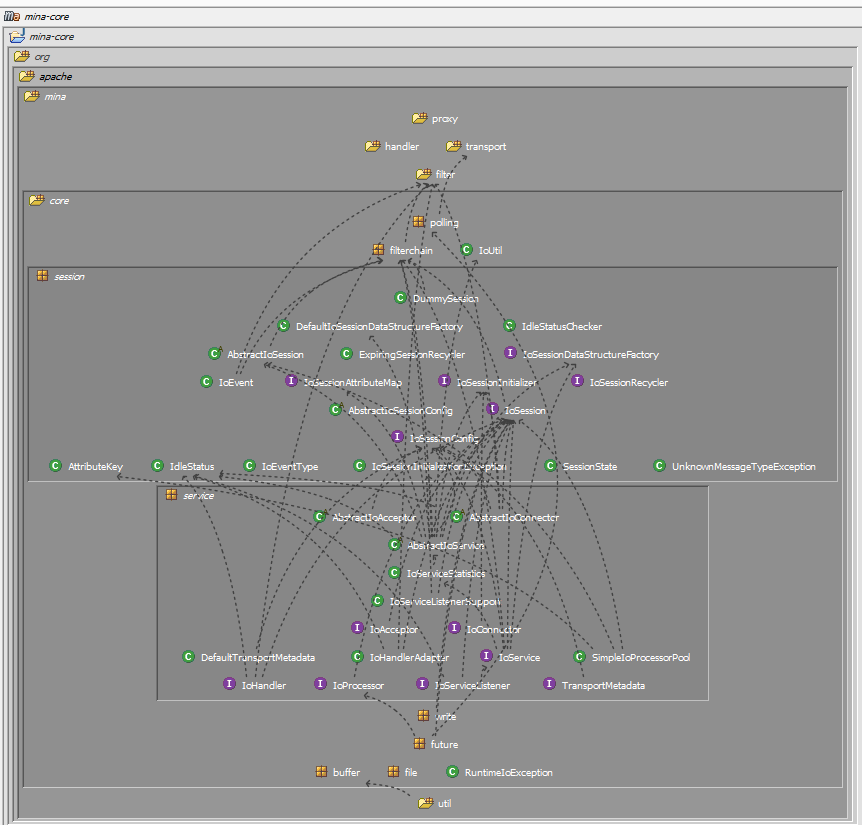
\includegraphics[scale = 0.7]{images/MINA_core_core_initial.png}
    \caption{Structure of the \texttt{mina-core-core} module.}
    \label{fig:mina_core_core_initial}
\end{figure}

\begin{figure}[H]
    \centering
    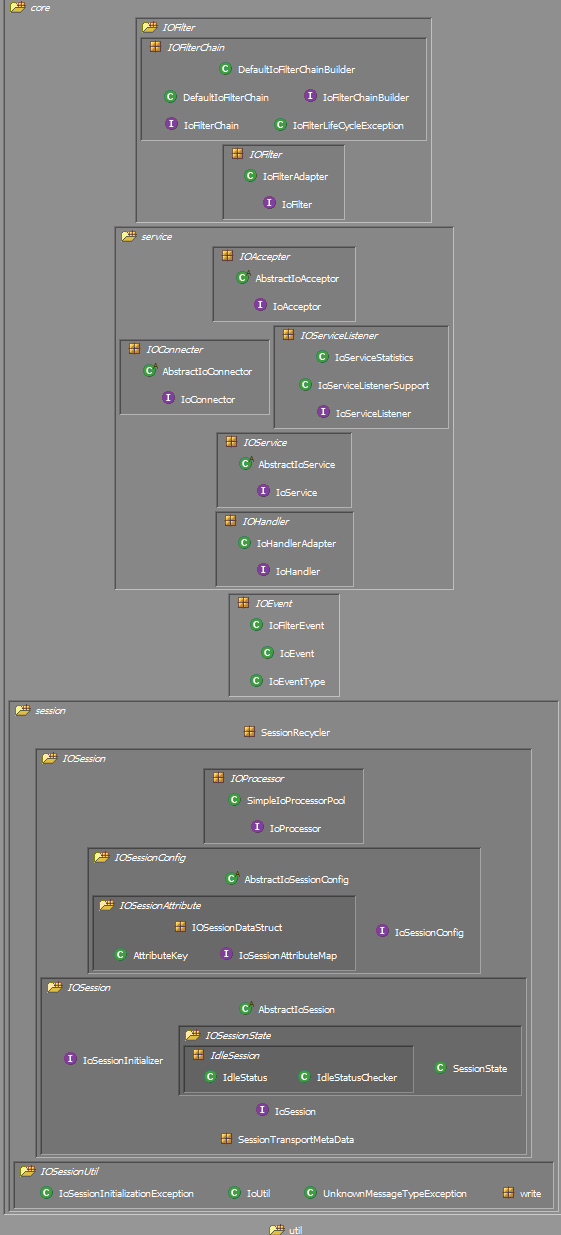
\includegraphics[scale=0.7]{images/MINA_core_core_restructured.png}
    \caption{Restructured \texttt{mina-core-core} module.}
    \label{fig:mina_core_core_restructured}
\end{figure}

\begin{figure}[H]
    \centering
    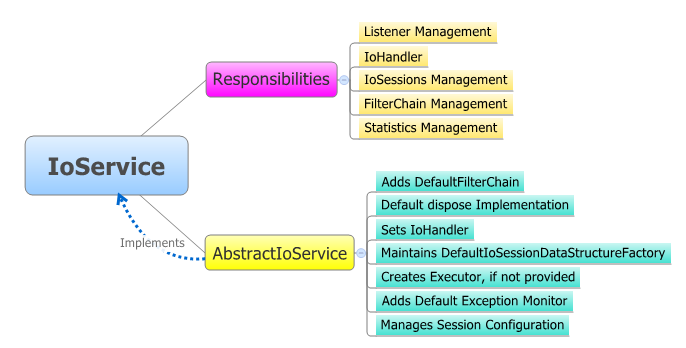
\includegraphics[width=\textwidth]{images/IoService_mindmap.png}
    \caption{Overview of the responsibilities of the \texttt{mina-core-core-service} component extracted from \cite{mina-userguide}.}
    \label{fig:service_responisbilities}
\end{figure}

\begin{figure}[H]
    \centering
    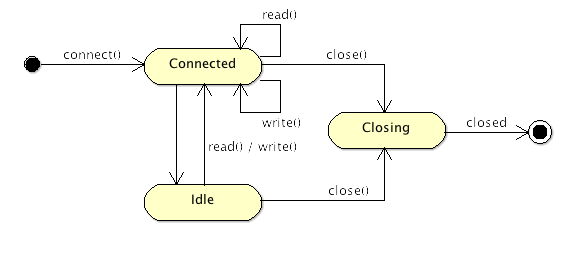
\includegraphics[width=\textwidth]{images/session-state.png}
    \caption{Visualisation of a session's life cycle, capturing the possible session states, extracted from \cite{mina-userguide}.}
    \label{fig:session_lifecycle}
\end{figure}


\subsection{MINA integration}

\begin{figure}[H]
    \centering
    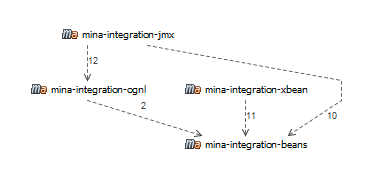
\includegraphics{images/MINA_integration_dependencies.png}
    \caption{MINA integration packages dependencies}
    \label{fig:dependencies_integration}
\end{figure}

\begin{figure}[H]
    \centering
    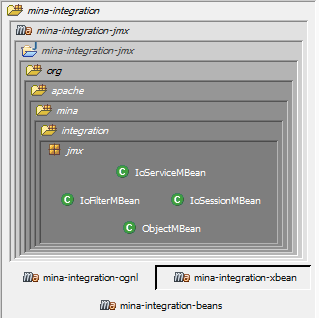
\includegraphics[width=0.5\textwidth]{images/MINA_integration_jmx.png}
    \caption{MINA JMX integration package}
    \label{fig:jmx_integration}
\end{figure}

\begin{figure}[H]
    \centering
    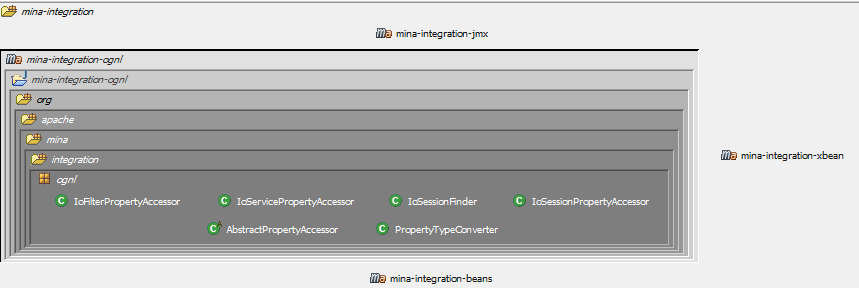
\includegraphics[width=\textwidth]{images/MINA_integration_ognl.png}
    \caption{MINA OGNL integration package}
    \label{fig:ognl_integration}
\end{figure}

\begin{figure}[H]
    \centering
    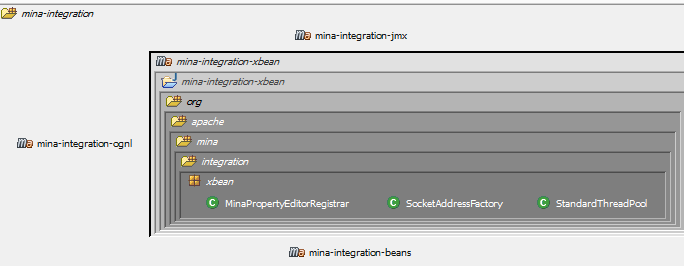
\includegraphics[width=\textwidth]{images/MINA_integration_xbean.png}
    \caption{MINA XBean integration package}
    \label{fig:xbean_integration}
\end{figure}

\begin{landscape}
\begin{figure}
    \centering
    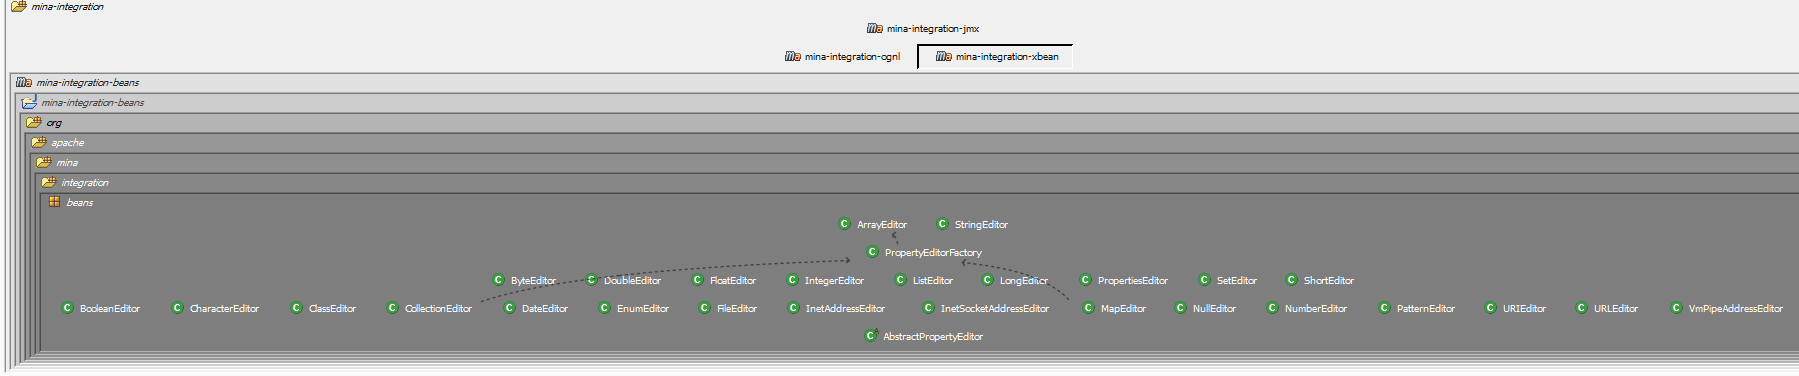
\includegraphics[scale=0.5]{images/MINA_integration_beans.png}
    \caption{MINA Beans integration package}
    \label{fig:beans_integration}
\end{figure}
\end{landscape}

\subsection{MINA state machine}

\begin{figure}[H]
    \centering
    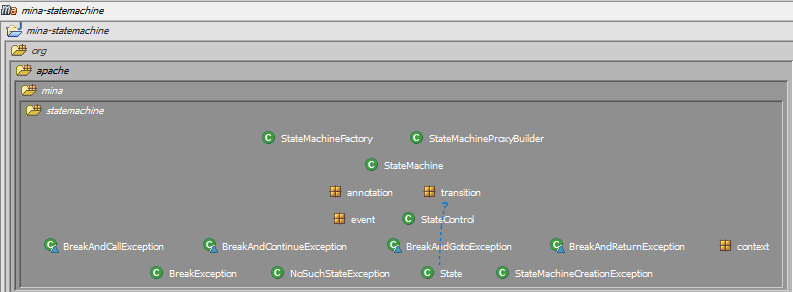
\includegraphics[width=\textwidth]{images/MINA_structure_statemachine_initial.png}
    \caption{Structure of the \texttt{statemachine} package}
    \label{fig:statemachine_initial}
\end{figure}

\begin{figure}[H]
    \centering
    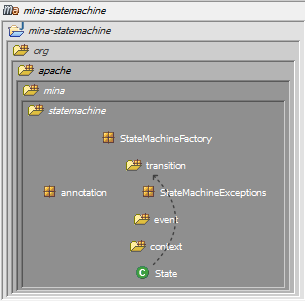
\includegraphics[width=0.7\textwidth]{images/MINA_structure_statemachine_restructured.png}
    \caption{Overview of the \texttt{statemachine} package after restructuring}
    \label{fig:statemachine_restructured}
\end{figure}

\begin{landscape}
\begin{figure}
    \centering
    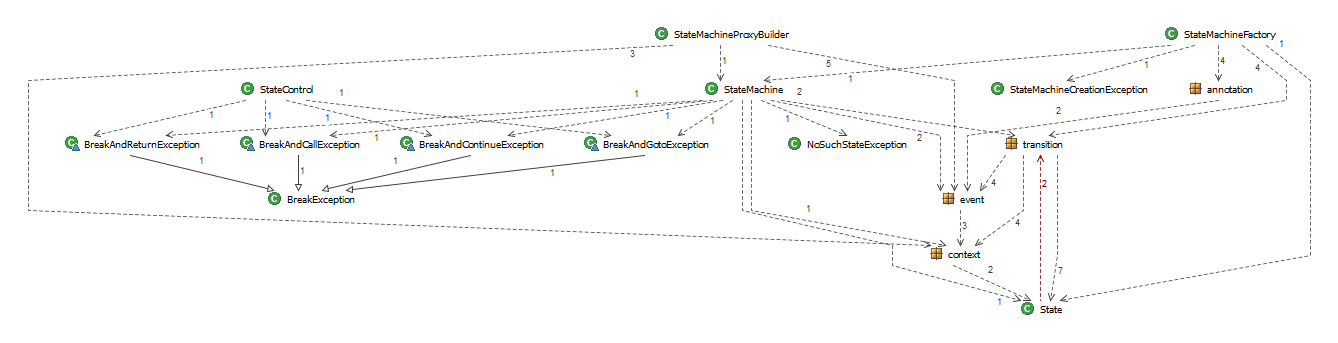
\includegraphics[scale = 0.5]{images/MINA_dependencies_statemachine_initial.png}
    \caption{Inner dependencies of the \texttt{statemachine} package}
    \label{fig:statemachine_initial_dependencies}
\end{figure}
\end{landscape}

\begin{figure}[H]
    \centering
    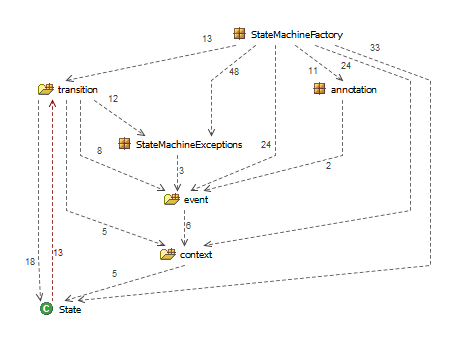
\includegraphics[scale = 0.8]{images/MINA_dependencies_statemachine_restructured.png}
    \caption{Inner dependencies of the \texttt{statemachine} package after restructuring}
    \label{fig:statemachine_restructured_dependencies}
\end{figure}

\begin{figure}[H]
    \centering
    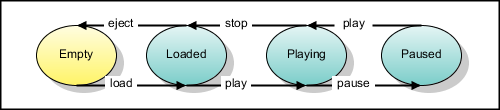
\includegraphics[width=\textwidth]{images/state-diagram.png}
    \caption{A simple example of a state application which can be implemented using the state machine functionality of MINA; the example has been extracted from \cite{mina-userguide}.}
    \label{fig:statemachine_example}
\end{figure}

\subsection{MINA HTTP}

\begin{figure}[H]
    \centering
    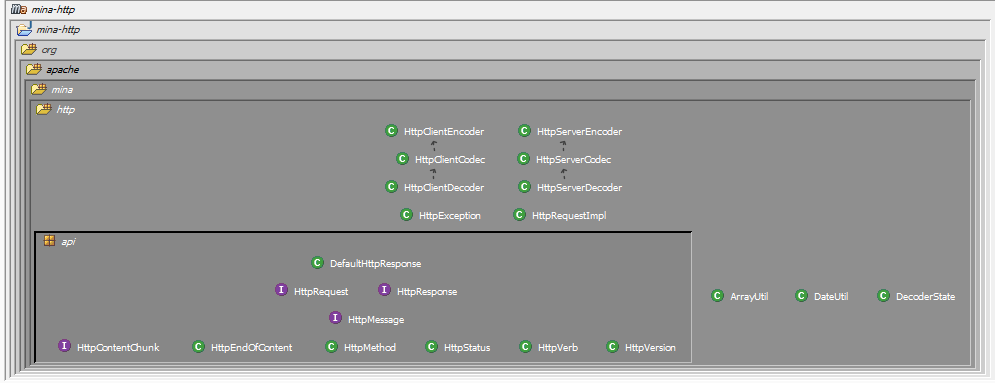
\includegraphics[width=\textwidth]{images/MINA_http_structure_initial.png}
    \caption{Structure of the \texttt{http} package}
    \label{fig:http_structure_initial}
\end{figure}

\begin{figure}[H]
    \centering
    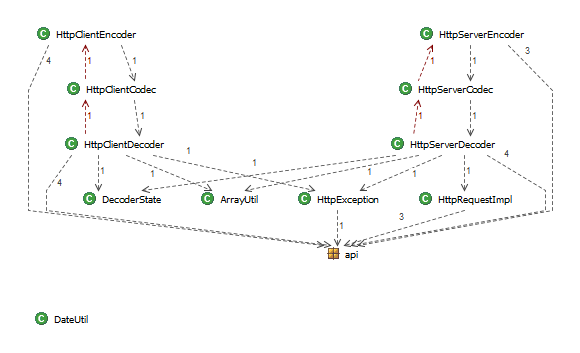
\includegraphics[width=\textwidth]{images/MINA_http_dependencies_initial.png}
    \caption{Inner dependencies of the \texttt{http} package}
    \label{fig:http_dependencies_initial}
\end{figure}

\begin{figure}[H]
    \centering
    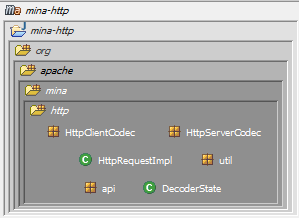
\includegraphics{images/MINA_http_structure.png}
    \caption{Overview of the restructured \texttt{http} package}
    \label{fig:http_structure_restructured}
\end{figure}

\begin{figure}[H]
    \centering
    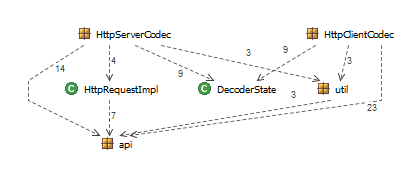
\includegraphics{images/MINA_http_dependencies.png}
    \caption{Inner dependencies of the restructured \texttt{http} package}
    \label{fig:http_dependencies_restructured}
\end{figure}

\subsection{MINA transport APR}

\begin{figure}[H]
    \centering
    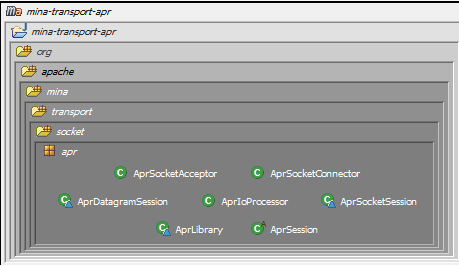
\includegraphics{images/MINA_apr_structure.png}
    \caption{Structure of the \texttt{transport-apr} package}
    \label{fig:apr_structure}
\end{figure}

\begin{figure}[H]
    \centering
    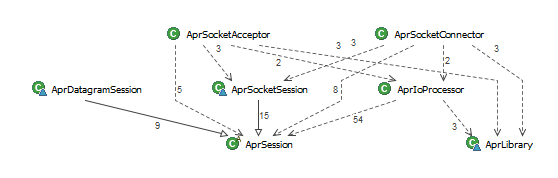
\includegraphics[width=\textwidth]{images/MINA_apr_dependencies.png}
    \caption{Inner dependencies of the \texttt{transport-apr} package}
    \label{fig:apr_dependencies}
\end{figure}

\section{Call graphs for methods included in the create server use case}
\label{sec:call_graphs}

\begin{figure}[H]
    \centering
    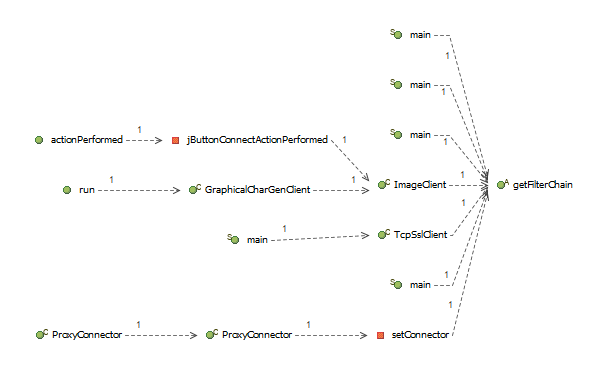
\includegraphics[width=\textwidth]{images/getfilterchain.png}
    \caption{\texttt{getFilterChain} call graph}
    \label{fig:getfilterchain}
\end{figure}
\begin{figure}[H]
    \centering
    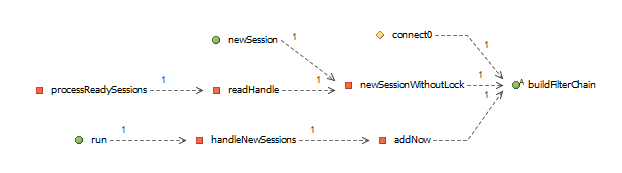
\includegraphics[width=\textwidth]{images/buildfilterchain.png}
    \caption{\texttt{buildFilterChain} call graph}
    \label{fig:buildfilterchain}
\end{figure}

\begin{figure}[H]
    \centering
    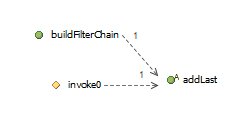
\includegraphics{images/addlast.png}
    \caption{\texttt{addLast} call graph}
    \label{fig:addlast}
\end{figure}

\begin{figure}[H]
    \centering
    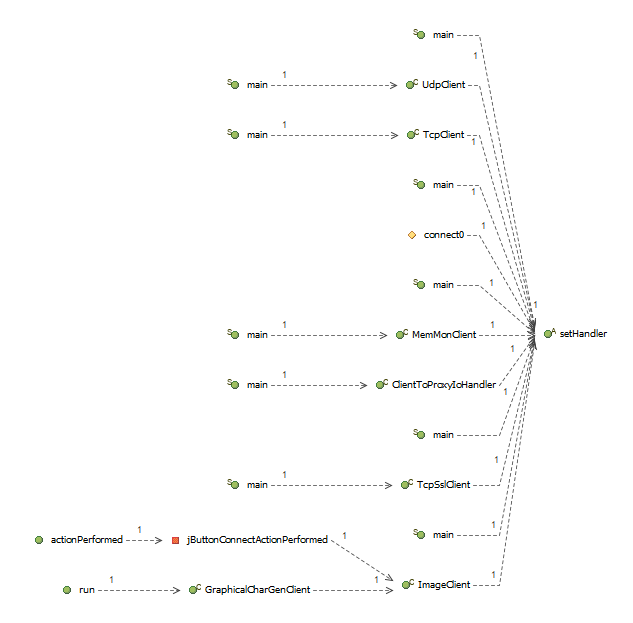
\includegraphics[width=\textwidth]{images/sethandler.png}
    \caption{\texttt{setHandler} call graph}
    \label{fig:sethandler}
\end{figure}

\begin{figure}[H]
    \centering
    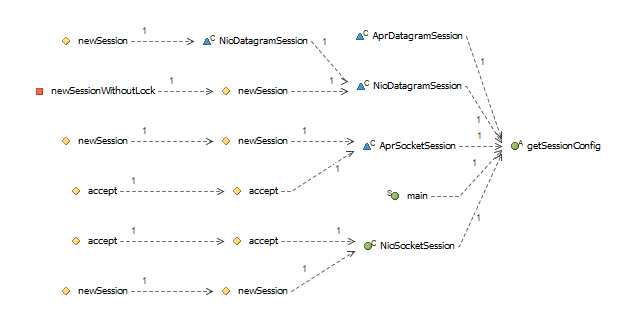
\includegraphics[width=\textwidth]{images/getsessionconfig.png}
    \caption{\texttt{getSessionConfig} call graph}
    \label{fig:getSessionConfig}
\end{figure}


\begin{figure}[H]
    \centering
    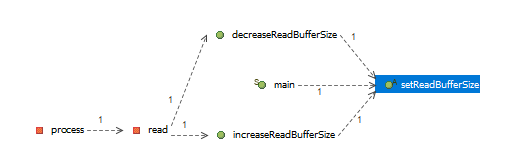
\includegraphics[width=\textwidth]{images/setreadbuffersize.png}
    \caption{\texttt{setReadBufferSize} call graph}
    \label{fig:setreadbuffersize}
\end{figure}

\begin{figure}[H]
    \centering
    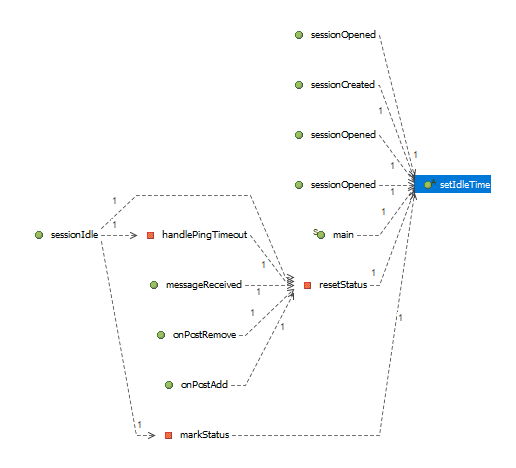
\includegraphics[width=\textwidth]{images/setidletime.png}
    \caption{\texttt{setIdleTime} call graph}
    \label{fig:setidletime}
\end{figure}









